\chapter{Implementation}

In this chapter, we share our experience of how implementation is planned and being done.

\section{Big Picture}

Indico has a complex product with many features. As a result, Indico is a big code base which is easily seen table \ref{loc_comparison} in comparison to some popular services.

Due to complexity, it isn't possible to change database instantly. Since we would like to see the result of our changes all the time, we need a working system. Therefore, main database machinery, firstly, is integrated and then each modules is refactored into using new database. At the same time, tests are being written to validate the behaviour of code. After one module is ready, it will be pushed into production to be tested there, too while other modules are being refactored.



\section{Scope of Project}

When ZODB started to perform badly, incremental optimizations were done. For instance, Room Booking - enables location and room management, and reserving rooms for events, is one of the most complex and involving modules and it's separated into its own database. Since it's not very tightly integrated into main database, it is the first module as a good starting point to get experience in refactoring, frameworks, tool chain and interpolate complexity.

\section{Room Booking Schema}

Since we are going to use a RDBMS, schema must be designed up-front.

We started to inspect database with external tools to get the object structure. However, ZODB is an object database, inspection database without their mapped run-time classes is much more difficult to relational databases. Even if there are 3 available tools , non of them is stable and well-supported:
\begin{itemize}
  \item zodbbrowser
  \item eye
  \item z3c.zodbbrowser (unfinished GSOC project)
\end{itemize}

We have tried all of them but \textit{eye} was the most stable to our experience but even \textit{eye} couldn't open our production database which is around 30 GB after one day of interaction, get biggers with every update to objects since storage mechanism of ZODB is to save every version of objects and only to put a reference to the latest version.

Viewer may be patched but responses with developer of module back and forth were slow and since we don't want to lose time with it, we worked with only empty database at first. We loaded data incrementally by testing to find the tipping point where it fails. Next logical step is to analyse the mapped classes which isn't an easy task because we are talking about classes composed of $\sim$2000 lines.

\hspace{-0.65cm}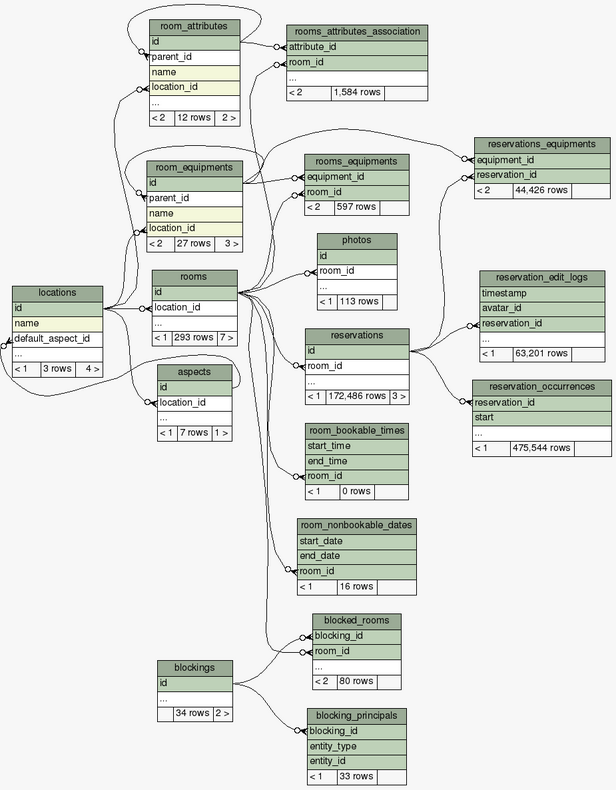
\includegraphics[scale=0.63]{6/figures/schema.png}

It's a bit challenge because classes in ZODB uses \textit{set}, \textit{list}, \textit{dictionary} data structures of Python and there are places where data is replicated within objects. They should be fully normalized into their own tables.

There are places which work nicely in small number of cases but don't scale:
\begin{itemize}
  \item Repetition enumeration for reservations: currently, there are only 6 options so their text representations and dates are calculated explicitly. Moreover, their implementation doesn't do what their description says. Adding one more repetition type isn't easy so their text and date generation must be humanized and automated.
  \item Location and Room attributes and equipments: These are replicated for each one, they all mean the same thing, though.
  \item Location and Room attributes and equipments: They have a hierarchy but this hierarchy is hard coded into source code. Each level of hierarchy is one list in room object, for instance.
  \item Location and Room attributes and equipments: Due to replication, there are inconsistencies. Room can't have an equipment which its location doesn't have but since there is no check, it's possible.
  \item Reservation repetitions are materialized. Reservation objects keep track of start and end date with repetition type. Whenever reservation request has come, these repetitions are generated in client and they're checked for overlap with the requested time span.
\end{itemize}

In addition to refactoring to use new database, these problems are also addressed with new schema.

Finally, some helper scripts are implemented to easily generate a graph of schema and \textit{UML} diagram of classes. Understanding what is what from code inspection as a start may be time wasting. Hopefully, these scripts will same some time later by providing a high level of system. Actually, analysis of ZODB comes from lack of tools. In RDBMS, especially PostgreSQL, pgAdmin makes this kind of inspection much easier.

\section{ORM - Object Relational Mapper}

We are dealing with objects and RDBMS is waiting pure serialized binary data. This may be solved by ourselves but there are stable object relational mapper libraries for Python:
\begin{itemize}
  \item SQLALchemy
  \item Django ORM
  \item pony
  \item peewee
  \item Storm
\end{itemize}

We have chosen SQLAlchemy. Django ORM would be a ridiculous idea without Django web framework. Storm is developed at Canonical and has shown capabilities in Launchpad scale but other than that, there aren't many . pony and peewee have a smaller user community and less features compared to SQLAlchemy.

SQLAlchemy is a very stable library approaching its $1.0$ major version and preferred by Mozilla, Nasa, OpenStack. Some of its nice features are:
\begin{itemize}
  \item Architecture: SQLAlchemy is composed of two layers, core and orm. Orm layer makes easier to play with objects but more fine-grained control is tuned by core layer.
  \item Declarative DDL, Data Definition Language.
  \item Unit of work: SQLAlchemy prevents excessive talking to database, instead everything is put into queues and batched in one go.
  \item Powerful query generation: SQL construction from Python functions and expressions.
  \item Modular and extensible: Custom types, custom compile of queries.
  \item Eager/Lazy loading and caching
\end{itemize}

Morever, Flask, micro-web framework, recently is integrated into Indico. Before Flask, Indico has a custom request handle and dispatch mechanism. Even if it's done by Flask now, Flask isn't fully utilized. We added Flask-SQLAlchemy to our arsenal with SQLAlchemy to more tight integration of Flask into Indico.

\section{MVC - Model View Controller}

Indico isn't as modular as it should be. Every function related to one layer is put into the same file. For example, in Room Booking module, each request handler is in the same file so this file is huge, $\sim$15000 lines. Navigating, understanding and editing it is difficult. Even text editor may sometimes freeze while editing such a big file.

Since we're refactoring, why don't we make our lives easier for the future? MVC, model-view-controller, pattern is a well-known software pattern to divide applications into interconnected parts. MVC enables separation between how data is represented within system, how requests are handled and how data is shown to users.

We are adapting MVC pattern as refactoring for new database so as to have manageable pieces.

\section{Models}

We use SQLAlchemy and Flask-SQLAlchemy and their declarative DDL. 

Firstly, one SQLAlchemy object for database interface is put into \textit{indico.core.db}. This object makes table and type primitives available.

Secondly, each model is put into its own file. After importing \textit{db} object, each class member is set to  a column object with specific type from \textit{db} object.

At runtime, after Flask application is created, \textit{db} object is imported and configured. Flask-SQLAlchemy comes with reasonable defaults. However, \textit{db} is configured with values retrieved from main Indico config object which contains Flask-SQLAlchemy defaults at default.

After getting an application context from flask application and setting application of \textit{db} object to this application, each model that is using SQLAlchemy should  be imported to resolve interdependence between models. At this time, we can drop existing database and/or create database. Models are ready to use.

\section{Distributed Queries}

ZODB isn't dropped at one night so RDBMS and ZODB should coexist until complete transition is done. Therefore, distributed queries must be supported. If one of databases gives error, transaction must be aborted and state must be roll-backed to previous status.

We may develop this functionality ourselves but luckily, SQLAlchemy provides extensibility for \textit{session} object which is the interface to the \textit{db} object and local cache. Therefore, adding /removing objects to/from \textit{session} may be done by application developer while commit/roll-back is called by extension. Moreover, ZODB transaction module can manage external transactions in addition to its own ZODB transaction with a helper that provides a common ZODB interface. Architectures of these libraries is nicely fits into structured Indico request handler hierarchy. Every request handler extends \textit{base} request handler which is the only point where transactions are committed or roll-backed.

To make this design possible, we use \textit{zope.sqlalchemy} which is a joint effort of ZODB and SQLAlchemy developers. Making \textit{base} request handler only responsible, developers aren't needed to deal with transaction logic any where else, they only manipulate objects, instead and \textit{base} request handler handles the rest because when a request has come, one thread-local \textit{session} is created and one transaction is started. Developer uses this \textit{session} to implement application logic and at the end, \textit{base} request handler checks session for changes. If there are changes, they have been tried to be committed  . If everything goes well, results are show, otherwise transaction is roll-backed and appropriate error message is displayed. Finally, transaction is finalized and  thread-local \textit{session} is closed which means request has ended.

There is a subtle detail because \textit{db} object must be created with that \textit{zope.sqlalchemy} extension. However, we don't always need that extension such as migration scripts (ZODB $\rightarrow$ RDBMS) and unit tests. When it's used unless needed, it causes more troubles than benefits so dynamic loading of \textit{db} object is needed. Since \textit{db} object is the main building of database, it's in use literally everywhere. The only logical place to add this capability is \textit{indico.core.db}. It's implemented by malleability of Python. Caller modules set \textunderscore \textunderscore \textit{no}\textunderscore \textit{session}\textunderscore \textit{options}\textunderscore\textunderscore\textit{ }global to \textit{true}. While \textit{db} is being loaded, \textit{db} module checks that specific global in frames, call stack, of parent modules. If global is seen, then pure vanilla SQLAlchemy object is imported without any extension. Otherwise, it is loaded with ZODB transaction extension.

\section{Queries}

In ZODB, accessing objects and their properties are easy but inefficient. Even if a small property of an object is needed, we need to load whole object and then access its property. There is no possibility of doing projections. As said in discussion of database types, object is seen a big blob from the point of view of database.

Even worse, since we can't load object in batches in ZODB, there must be multiple back and forth connections between server and client. In terms of performance, this connection should be minimized into one.

Relational databases helps us to overcome these problems at the expense of an increase query complexity and portability between different databases.

\subsection{Complexity}

In ZODB, main implementation is to get all objects one by one while doing filtering and computation on client with retrieved object and putting it into result set if it satisfies. Some tricks are already implemented to efficiently get objects such as indexes. If every reservation within one particular day, for example, is put into a Python list, all reservations can be loaded easily for requesting that list. This computation is \textit{pre-map-reduce} era such that data is brought for code. It should have been the other way, moving code to data, since costly one is moving data like favoured by \textit{map-reduce} paradigm.

In RDBMS, we can create a huge filter, query, and send it to server where data lives and get back only what is needed to satisfy the request. Since schema is fully normalized, accessing data requires joins and combining different types of data to make only one request to the database server.

For example, to show booking interface to user, rooms and their capacity are needed but also max capacity should be known to initialize filters. There are two options:
\begin{itemize}
  \item Getting all rooms and then iterating over them and finding max in client
  \item Getting all rooms and max capacity at the same time from server
\end{itemize}

First option is easier but not efficient as much as it could be. Second option is blazingly fast since database has already an index on capacity such that there is no need for computation, it's only one look-up. However, retrieving rooms and one integer in the same result is hard because each record should have same structure which is \textit{not}. To get all into same structure, max capacity should be faked into a room object. 

Another example may be showing availabilities of rooms in some time span because a tree-like structure should be retrieved from server in one go such that there may be multiple rooms with multiple reservations within one day. Since it's favourable to return one record for each day, rooms and their reservations must be aggregated somehow. However, this aggregation isn't a simple SQL function like \textit{min} and it's more similar to concatenating records. Making this aggregation without powerful types supported by database such as \textit{array} in \textit{PostgreSQL} to keep queries portable loses type information.

As in examples, there is a trade-off between performance and complexity. As it gets more performant, it gets more complex. However, queries are written once and updated occasionally but they are run frequently. That's why performance is chosen over complexity.

\subsection{Portability}

Making queries better in terms of performance requires us to optimize for one database. This breaks portability because some aggregation function supported in PostgreSQL isn't available in MySQL, for instance. Using SQLAlchemy abstracts database but if specific extensions and types are utilized, then it's hard plug and play a different database. Likely, SQLAlchemy is extensible and provides a compiler to be extended.

For example, we would like to aggregate one column into an array in PostgreSQL with \textit{array\textunderscore agg} method. However, this method isn't available in MySQL so it'll cause an error. Compiler provided by SQLAlchemy generates custom SQL for each database. If we write an \textit{array\textunderscore agg} compiler construct and we can supply with information to call default \textit{array\textunderscore agg} on PostgreSQL and do custom string concatenation on MySQL to get the similar result.

Main goal is to prevent ourselves from using specific methods and types as much as possible and when it's not possible, one compiler construct for respective method is provided. Even if we try not to diverge from common features, queries are optimized for PostgreSQL since it'll be production environment at the end.

\section{Testing}

A complex system is getting more complex by entering into a transition phase in which many libraries are being integrated. Thus, unit tests are required to validate that same functionality as refactoring has been kept. Flask and its ecosystem are being more utilized in Indico so we chose using \textit{Flask-Testing} to write unit tests.

\textit{Flask-Testing} automatically populates and drops database for each to decrease coupling between tests. Due to the usage of \textit{Flask-SQLAlchemy}, we should be in \textit{app\textunderscore context} or \textit{test\textunderscore request\textunderscore context} which mean that application must be set for \textit{db} object or one request should be qoing on, respectively. \textit{Flask-SQLAlchemy} provides \textit{test\textunderscore request\textunderscore context}, creation and dropping of \textit{session} for us.

\section{Controllers}

Controllers are moved into their new place, \textit{indico.modules.rb.controllers} and divided into small self-contained packages such that:
\begin{itemize}
  \item admin
    \begin{itemize}
      \item locations
      \item rooms
      \item reservations
    \end{itemize}
  \item user
    \begin{itemize}
      \item locations
      \item rooms
      \item reservations
      \item blockings
    \end{itemize}
  \item decorators
  \item forms
  \item mixins
  \item utils
\end{itemize}

There are two main packages; namely, \textit{admin} and \textit{user}. Under each one of them, specific controllers are laid out. Common functionality is put into top level such as decorators, form classes and utility methods.

With this structure, navigation within code base is faster and since related functionality is clustered in one small file, finding one piece of information is quickier.

\subsection{Forms}

Most complexity of controllers code comes from validation of form fields. No form library is utilized and validation of each field manually which is repetitive and error-prone. Since huge body of controllers is changing, field validation may also be off-loaded to 3rd party form library.

The most popular and stable library for forms is \textit{WTForms} and we used it with Flask and SQLAlchemy extensions to automate validation.

Request handlers in Indico has mainly 3 important methods:
\begin{itemize}
  \item authorization check: put into package base nicely
  \item parameter check: used to create a respective form object and validate
  \item process: generates response by using validated form data
\end{itemize}

Controllers are light-weight because nice package structure enabled to get authorization check out of picture. Process is implemented as one query in appropriate model. Now, with integration of WTForms, parameter check is delegated. As a result of these transformations, controllers composed of hundreds lines of code is now a simple glue between models and forms.

WTForms provides:
\begin{itemize}
  \item A declarative language for fields as SQLAlchemy does for models.
  \item Type casting and many default validators as well as ability to write custom validators
  \item Custom types
  \item Automatic \textit{CSRF} protection which isn't used since Indico has already protection in a higher level.
\end{itemize}

\subsection{More Flask}

Flask is integrated into Indico because
\begin{itemize}
  \item there was a legacy hard-coded request dispatch mechanism which should be automated and extensible
  \item custom solution of Indico was like reinventing the wheel which is costly in terms of time and money
  \item custom solution is hard-coded which is repetitive and error-prone by nature but Flask creates an abstraction layer to easily manage URLs and is more resistant to errors.
  \item Flask does automatic type validation and conversion for URL params
  \item Flask provides better compatibility with low-level WSGI server implementation.
  \item All of the previous enables beautiful URLs which are better for users to remember as well as crawlers for SEO, search engine optimization.
  \item Flask provides powerful thread-local \textit{flash}, \textit{request} and \textit{session} objects to show messages to users, to access request related information and to access all data for the current user, respectively. 
\end{itemize}

Even if Flask could bring above features, it's just a facade between WSGI and Indico custom request handler logic because it's only used for URL mapping. For instance, request handlers get their request data as parameters from base request handler by copying. This is unnecessary since request handlers are already able to access request data from \textit{flask.request}. While base request handler is being refactored for distributed queries, it's also updated to pass request data conditionally so that new request handlers have a simpler signatures and access their data from \textit{flask.request} while keeping compatibility with old ones.

Parameters are passed back and forth to notify users for action success or fail. Interface shows respective message according to action status. However, in refresh, since parameters are a part of URL, same message will be displayed again which is misleading and ugly. Therefore, new request handlers use \textit{flask.flash} to show messages only one and getting rid of parameter navigation clutter.

\section{Views and Templates}

The same structure of controllers is replicated under views. That enables easy navigation and more understandable code base such that if there is a request handler in \textit{indico.modules.rb.controllers.x.y.z}, its respective view is simply in \textit{indico.modules.rb.views.x.y.z}.

Templates are mainly updated to keep consistency and naming scheme. However, in some interface, there were legacy inefficient JavaScript and old widgets that may be better to change for consistent user interface. Pure JavaScript is mostly rewritten in \textit{underscore.js} to offload browser quirks to library and have a modern, concise code since it's already in use. Old widgets are replaced by jQuery UI widgets such as \textit{DatePicker}.

\subsection{Unicode}

Mako template engine (developed by main SQLAlchemy developer) is in production at Indico and Mako provides an option to disable Unicode explicitly. Until now, fields are Python byte strings and internationalization engine returns UTF-8 encoded strings so currently templates don't support unicode objects. Using deeply Flask and SQLAlchemy makes transition to Python 3 faster by using unicode objects everywhere but until that time, refactored modules, room booking for now, differs from rest. Location, room or reservation objects can't be passed directly templates. Their properties must be converted into byte string by encoding before generating result.

This problem can be solved in two ways:
\begin{itemize}
  \item Calling encode on properties whenever it's written into template
  \item Writing a custom template to encode unicode objects and setting it as first default filter in template engine
\end{itemize}

First one is verbose and error-prone so second one is chosen not to bother developers with a bad result of transition phase. Second implementation is worse in terms of performance but pros and cons are compared, it weighs heavier such that a new developer that isn't informed about this quirk may not be aware of it.

In overall, ZODB version wasn't supporting Python 3 so getting rid of main dependency of Indico and tight integration of Flask, WTForms and SQLAlchemy are a huge push for the adaptation of Python 3 in Indico.